\section{Introduction}

The wiring of cortical circuits is highly dynamic. Spine sizes fluctuate even in the absence of neural activity and there is constant synaptic turnover \cite{Loewenstein2015}. In models of cortical circuits, two major mechanisms are typically considered to drive the efficacies of synaptic connections: Spike-timing dependent plasticity (STDP) is often assumed to strengthen or weaken synaptic connections in an additive manner, independent of the current weight. Synaptic normalization, on the other hand, acts multiplicatively on synapses by scaling their efficacies by a varying factor that depends on the availability of synaptic resources \cite{Triesch2017} (see Fig.~\ref{fig:spines}).



\begin{center}\vspace{0.5cm}
  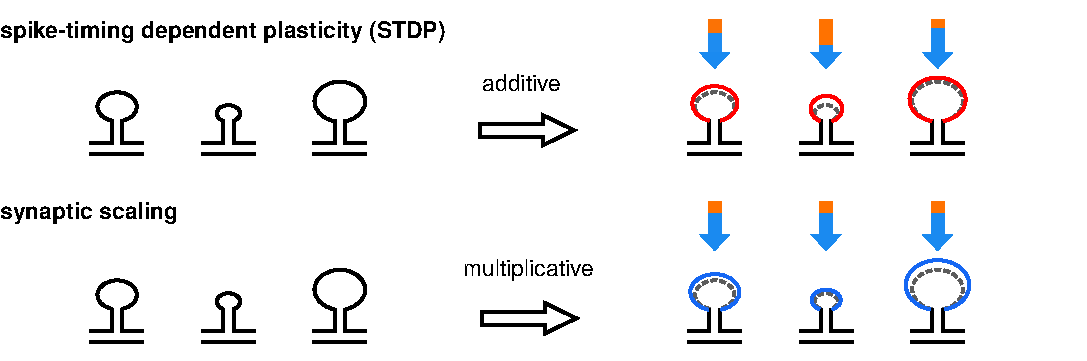
\includegraphics[width=\columnwidth]{%
    /home/fh/pub/graphics/synapse_size_dynamics/synapse_size_dynamics.png} %
  \captionof{figure}{Spike-timing dependent plasticity changes synaptic efficacies additively, while synaptic normalization acts multiplicatively on the synaptic weights.}
  \label{fig:spines}
\end{center}\vspace{2cm}


To model the fluctuations of synaptic spine sizes over time, a stochastic process called Kesten process has been suggested \cite{Kesten1973, Statman2014}. In this process, a random variable $X_n$ at time step $n$ is updated by scaling it with a random multiplicative factor $a_n$ and then adding a random increment $b_n$ according to
%
\begin{align}
  X_{n+1} = a_n X_n + b_n. \label{eq:kesten}
\end{align}
%
This stochastic model has been successfully used to describe the distribution of synaptic spine sizes measured in experiments. Here we extend the Kesten process by including the explicit creation and elimination of spines. Simulation and analysis of the model reveals that the distribution of lifetimes approximately follow a power law, as has been recently identified in experiments in the rat neocortex \cite{Loewenstein2015}.


%% In an experimental study by \textcite{Loewenstein2015} chronic in-vivo two-photon imaging suggested that the lifetime dynamics of spines in the neocortex follow a power law. Motivated by results from detailed network simulations, we here consider a simple stochastic model based on the Kesten process in order to analyze how different properties of a cortical network might affect the lifetime distributions of synaptic spines.
